\documentclass[tikz,border=12pt]{standalone}
\usepackage{xcolor}
\usepackage{tikz}
\usetikzlibrary{shapes.geometric, arrows.meta, positioning, calc, backgrounds, fit, shadows}

\definecolor{k8sbg}{RGB}{245, 247, 250}
\definecolor{k8sborder}{RGB}{195, 207, 217}
\definecolor{configBg}{RGB}{230, 246, 240}
\definecolor{configBorder}{RGB}{46, 133, 94}
\definecolor{configText}{RGB}{30, 86, 61}
\definecolor{pvcBg}{RGB}{254, 244, 230}
\definecolor{pvcBorder}{RGB}{204, 116, 36}
\definecolor{pvcText}{RGB}{140, 72, 16}
\definecolor{jobBg}{RGB}{235, 243, 253}
\definecolor{jobBorder}{RGB}{59, 130, 246}
\definecolor{jobText}{RGB}{30, 64, 175}
\definecolor{serveBg}{RGB}{245, 238, 254}
\definecolor{serveBorder}{RGB}{147, 51, 234}
\definecolor{serveText}{RGB}{107, 33, 168}
\definecolor{svcBg}{RGB}{230, 248, 250}
\definecolor{svcBorder}{RGB}{14, 165, 233}
\definecolor{svcText}{RGB}{3, 105, 161}
\definecolor{clientBg}{RGB}{243, 244, 246}
\definecolor{clientBorder}{RGB}{107, 114, 128}
\definecolor{clientText}{RGB}{31, 41, 55}

\begin{document}
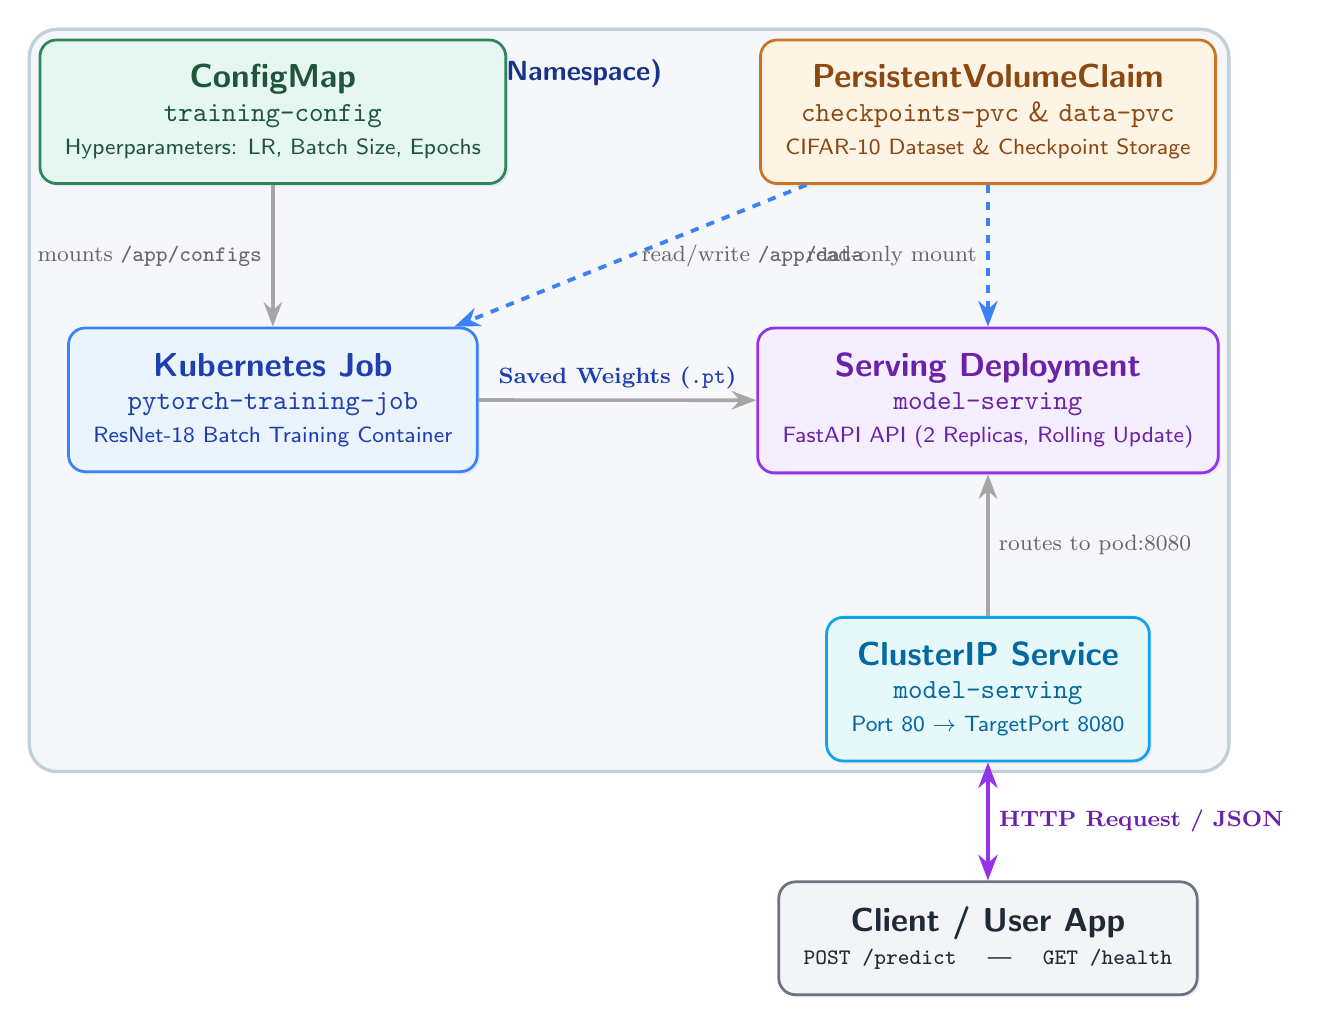
\begin{tikzpicture}[
    font=\sffamily,
    >=Stealth,
    node distance=2.2cm,
    clusterBg/.style={fill=k8sbg, draw=k8sborder, line width=1.2pt, rounded corners=10pt},
    card/.style={rounded corners=6pt, line width=1pt, align=center, inner sep=9pt, drop shadow={opacity=0.12, shadow xshift=1pt, shadow yshift=-1pt}},
    configBox/.style={card, fill=configBg, draw=configBorder, text=configText},
    pvcBox/.style={card, fill=pvcBg, draw=pvcBorder, text=pvcText},
    jobBox/.style={card, fill=jobBg, draw=jobBorder, text=jobText},
    serveBox/.style={card, fill=serveBg, draw=serveBorder, text=serveText},
    svcBox/.style={card, fill=svcBg, draw=svcBorder, text=svcText},
    clientBox/.style={card, fill=clientBg, draw=clientBorder, text=clientText},
    connArrow/.style={->, line width=1.3pt, draw=gray!70},
    dataArrow/.style={->, line width=1.4pt, draw=jobBorder, dashed},
    httpArrow/.style={<->, line width=1.4pt, draw=serveBorder}
]

    % Nodes
    \node[configBox] (config) {
        \textbf{\large ConfigMap}\\
        \texttt{training-config}\\
        \footnotesize Hyperparameters: LR, Batch Size, Epochs
    };

    \node[pvcBox, right=3.2cm of config] (pvc) {
        \textbf{\large PersistentVolumeClaim}\\
        \texttt{checkpoints-pvc} \& \texttt{data-pvc}\\
        \footnotesize CIFAR-10 Dataset \& Checkpoint Storage
    };

    \node[jobBox, below=1.8cm of config] (job) {
        \textbf{\large Kubernetes Job}\\
        \texttt{pytorch-training-job}\\
        \footnotesize ResNet-18 Batch Training Container
    };

    \node[serveBox, below=1.8cm of pvc] (serve) {
        \textbf{\large Serving Deployment}\\
        \texttt{model-serving}\\
        \footnotesize FastAPI API (2 Replicas, Rolling Update)
    };

    \node[svcBox, below=1.8cm of serve] (svc) {
        \textbf{\large ClusterIP Service}\\
        \texttt{model-serving}\\
        \footnotesize Port 80 $\rightarrow$ TargetPort 8080
    };

    \node[clientBox, below=1.5cm of svc] (client) {
        \textbf{\large Client / User App}\\
        \footnotesize \texttt{POST /predict} \quad | \quad \texttt{GET /health}
    };

    % Arrows
    \draw[connArrow] (config) -- node[left, font=\footnotesize, text=gray!80!black] {mounts \texttt{/app/configs}} (job);
    \draw[dataArrow] (pvc) -- node[right, font=\footnotesize, text=gray!80!black] {read/write \texttt{/app/data}} (job);
    \draw[dataArrow] (pvc) -- node[left, font=\footnotesize, text=gray!80!black] {read-only mount} (serve);
    \draw[connArrow] (job) -- node[above, font=\footnotesize\bfseries, text=jobText] {Saved Weights (\texttt{.pt})} (serve);
    \draw[connArrow] (svc) -- node[right, font=\footnotesize, text=gray!80!black] {routes to pod:8080} (serve);
    \draw[httpArrow] (client) -- node[right, font=\footnotesize\bfseries, text=serveText] {HTTP Request / JSON} (svc);

    % Background Box
    \begin{scope}[on background layer]
        \node[clusterBg, fit=(config) (pvc) (job) (serve) (svc), label={[anchor=north west, font=\bfseries\sffamily\color{jobText!80!black}, yshift=-8pt, xshift=12pt]north west:Kubernetes Cluster (\texttt{ml-training} Namespace)}] (cluster) {};
    \end{scope}

\end{tikzpicture}
\end{document}
